% Robocode AI Final Results Beamer Presentation
\documentclass[12pt,aspectratio=169]{beamer}

\usetheme{Madrid}
\setbeamertemplate{navigation symbols}{}
\setbeamertemplate{footline}[frame number]

\definecolor{mublue}{RGB}{0,51,102}
\definecolor{mugold}{RGB}{255,204,0}
\definecolor{codegray}{RGB}{245,247,250}
\definecolor{lightblue}{RGB}{228,240,252}
\definecolor{softgold}{RGB}{255,247,204}
\definecolor{goodgreen}{RGB}{39,124,86}
\definecolor{warnred}{RGB}{168,52,52}

\usecolortheme[named=mublue]{structure}
\setbeamercolor{title}{fg=white,bg=mublue}
\setbeamercolor{frametitle}{fg=white,bg=mublue}
\setbeamercolor{block title}{fg=white,bg=mublue}
\setbeamercolor{block body}{bg=codegray}
\setbeamertemplate{blocks}[rounded][shadow=true]

\usepackage[utf8]{inputenc}
\usepackage{graphicx}
\usepackage{xcolor}
\usepackage{tikz}
\usepackage{booktabs}
\usepackage{array}
\usepackage{colortbl}
\usetikzlibrary{arrows.meta,positioning,shapes.geometric,calc}

\graphicspath{{../logs/analysis/figures/}}

\setbeamerfont{frametitle}{size=\Large}
\setbeamerfont{title}{size=\LARGE}
\setbeamerfont{subtitle}{size=\large}
\setbeamerfont{normal text}{size=\large}
\setbeamerfont{itemize/enumerate body}{size=\large}
\setbeamerfont{itemize/enumerate subbody}{size=\normalsize}

\newcommand{\metric}[3]{%
  \begin{block}{#1}
    \centering {\Large\textbf{#2}}\\[-0.02cm]
    {\small #3}
  \end{block}
}

\title[Robocode Results]{AI in Robocode}
\subtitle{Bot-by-Bot Final Results from the Full Log Corpus}
\author[Becker \textit{et al.}]{
  Jacob  \and Adithya \and Dan \and
  Corbin \and Owen 
}
\institute{Misericordia University}
\date{April 28, 2026}

\begin{document}

{
  \setbeamertemplate{footline}{}
  \begin{frame}[plain]
    \centering
    \vspace{0.65cm}
    {\color{mublue}\Huge\textbf{AI in Robocode}}\\[0.25cm]
    {\large Bot-by-Bot Final Results}\\[0.35cm]
    {\color{mublue}\rule{0.78\textwidth}{0.8pt}}\\[0.4cm]
    {\normalsize
      Jacob  \quad$\cdot$\quad Adithya \\[0.18cm]
      Dan \quad$\cdot$\quad Corbin  \quad$\cdot$\quad Owen
    }\\[0.38cm]
    {\color{mublue}\rule{0.78\textwidth}{0.8pt}}\\[0.25cm]
    {\small Misericordia University \quad$\cdot$\quad CPS485 \quad$\cdot$\quad April 28, 2026}
  \end{frame}
}

\begin{frame}{Presentation Order}
\centering
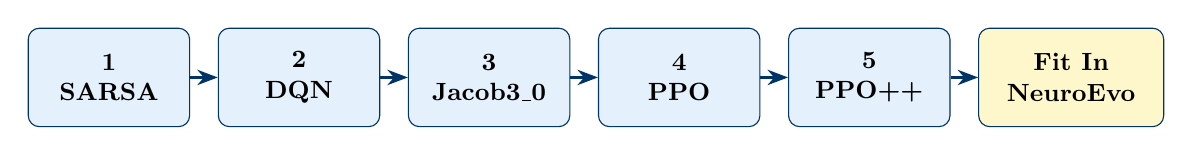
\begin{tikzpicture}[
  node distance=0.35cm,
  bot/.style={
    draw=mublue, fill=lightblue, rounded corners,
    minimum width=2.05cm, minimum height=1.25cm,
    align=center, font=\small\bfseries
  },
  extra/.style={
    draw=mublue, fill=softgold, rounded corners,
    minimum width=2.35cm, minimum height=1.25cm,
    align=center, font=\small\bfseries
  },
  arrow/.style={-{Stealth[length=2.6mm]}, thick, draw=mublue}
]
\node[bot] (sarsa) {1\\SARSA};
\node[bot, right=of sarsa] (dqn) {2\\DQN};
\node[bot, right=of dqn] (jacob) {3\\Jacob3\_0};
\node[bot, right=of jacob] (ppo) {4\\PPO};
\node[bot, right=of ppo] (ppop) {5\\PPO++};
\node[extra, right=of ppop] (neuro) {Fit In\\NeuroEvo};
\draw[arrow] (sarsa) -- (dqn);
\draw[arrow] (dqn) -- (jacob);
\draw[arrow] (jacob) -- (ppo);
\draw[arrow] (ppo) -- (ppop);
\draw[arrow] (ppop) -- (neuro);
\end{tikzpicture}

\vspace{0.45cm}
\begin{block}{Talk shape}
Each bot gets: idea, training evidence, benchmark result, and the one sentence we should remember.
\end{block}
\end{frame}

\begin{frame}{Evidence Corpus}
\begin{columns}[T,totalwidth=\textwidth]
\column{0.33\textwidth}
\metric{JSONL files}{167}{all current structured logs}
\column{0.33\textwidth}
\metric{Records}{251,273}{episodes, summaries, states}
\column{0.33\textwidth}
\metric{State rows}{102,094}{battle-state snapshots}
\end{columns}

\vspace{0.25cm}
\begin{itemize}
  \item Refreshed analysis: \texttt{summary\_20260428\_091712.json}.
  \item Structured logs came from training, evaluation, reward-curve, state-collection, PPO curriculum, and stress-test runs.
  \item Plain \texttt{.log} files were used for official Robocode scoreboards and failure notes.
\end{itemize}
\end{frame}

\begin{frame}{Shared Agent Loop}
\centering
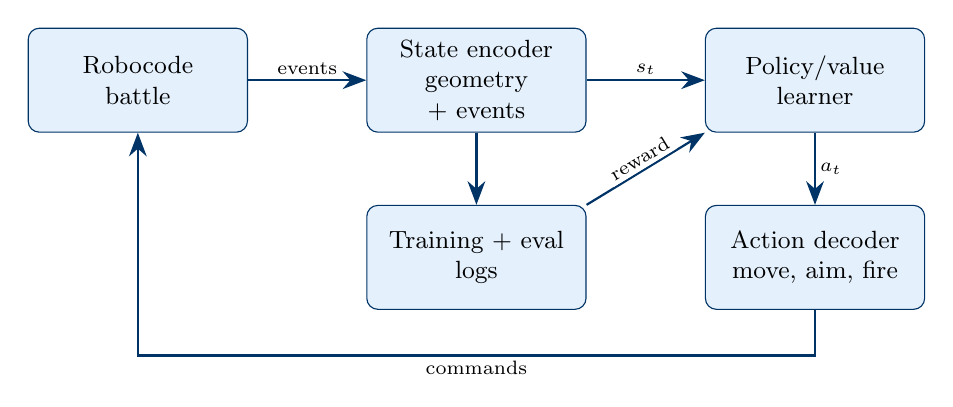
\begin{tikzpicture}[
  box/.style={
    draw=mublue, rounded corners, fill=lightblue,
    minimum height=1.32cm, text width=2.55cm, align=center, font=\small
  },
  arrow/.style={-{Stealth[length=3mm]}, thick, draw=mublue},
  lbl/.style={font=\scriptsize, fill=white, inner sep=1.5pt}
]
\node[box] (env) at (-4.3,0) {Robocode\\battle};
\node[box] (state) at (0,0) {State encoder\\geometry + events};
\node[box] (agent) at (4.3,0) {Policy/value\\learner};
\node[box] (logs) at (0,-2.25) {Training + eval\\logs};
\node[box] (action) at (4.3,-2.25) {Action decoder\\move, aim, fire};

\draw[arrow] (env.east) -- node[lbl, above] {events} (state.west);
\draw[arrow] (state.east) -- node[lbl, above] {$s_t$} (agent.west);
\draw[arrow] (agent.south) -- node[lbl, right] {$a_t$} (action.north);
\draw[arrow] (state.south) -- (logs.north);
\draw[arrow] (logs.north east) -- node[lbl, above, sloped] {reward} (agent.south west);
\draw[arrow] (action.south) -- ++(0,-0.58) -| node[lbl, near start, below] {commands} (env.south);
\end{tikzpicture}
\end{frame}

\begin{frame}{1. SARSA Bot}
\small
\begin{columns}[T,totalwidth=\textwidth]
\column{0.48\textwidth}
\begin{block}{On-policy table learning}
\small
\[
\delta_t=r_t+\gamma Q(s_{t+1},a_{t+1})-Q(s_t,a_t)
\]
\[
Q(s_t,a_t)\leftarrow Q(s_t,a_t)+\alpha\delta_t
\]
\end{block}
\begin{itemize}
  \item Simple, inspectable baseline.
  \item Learns from the action it actually takes next.
\end{itemize}

\column{0.52\textwidth}
\small
\begin{table}
\centering
\begin{tabular}{lrrr}
\toprule
\textbf{Scenario} & \textbf{Win} & \textbf{Survival} & \textbf{Damage} \\
\midrule
vs MeleeDQN & 100.0\% & 289.7 & 48.2 \\
vs PPOBot & 81.6\% & 188.6 & 72.8 \\
vs Jacob3\_0 & 43.8\% & 197.0 & 63.6 \\
Melee eval & 34.7\% & 370.1 & 162.7 \\
\bottomrule
\end{tabular}
\end{table}
\begin{block}{Remember}
SARSA was not the champion, but it was the best non-Jacob melee finisher.
\end{block}
\end{columns}
\end{frame}

\begin{frame}{2. DQN Bot}
\begin{columns}[T,totalwidth=\textwidth]
\column{0.52\textwidth}
\begin{block}{Deep Q-learning target}
\[
y_t = r_t+\gamma(1-d_t)\max_{a'}Q_{\bar\theta}(s_{t+1},a')
\]
\[
\mathcal{L}=\operatorname{SmoothL1}(Q_\theta(s_t,a_t),y_t)
\]
\end{block}
\begin{itemize}
  \item Neural value function instead of a table.
  \item Replay buffer and target network stabilize updates.
  \item This implementation struggled to convert state into offense.
\end{itemize}

\column{0.48\textwidth}
\small
\begin{table}
\centering
\begin{tabular}{lrrr}
\toprule
\textbf{Opponent} & \textbf{Win} & \textbf{Reward} & \textbf{Damage} \\
\midrule
Jacob3\_0 & 2.2\% & -8.965 & 0.0 \\
PPOBot & 4.4\% & -10.809 & 2.9 \\
SarsaBot & 4.8\% & -9.872 & 0.9 \\
Melee eval & 0.0\% & -10.954 & 4.0 \\
\bottomrule
\end{tabular}
\end{table}
\begin{block}{Remember}
The DQN idea was strong; this bot's learned behavior was not.
\end{block}
\end{columns}
\end{frame}

\begin{frame}{3. Jacob3\_0}
\small
\begin{columns}[T,totalwidth=\textwidth]
\column{0.43\textwidth}
\begin{itemize}
  \item DQN-based bot with the strongest final benchmark profile.
  \item Compact state vector: position, energy, walls, gun heat, enemy bearing/distance.
  \item Best at direct combat and still strong in multi-bot melee.
\end{itemize}

\column{0.57\textwidth}
\small
\begin{table}
\centering
\begin{tabular}{lrrrr}
\toprule
\textbf{Opponent} & \textbf{Win} & \textbf{Reward} & \textbf{Surv.} & \textbf{Damage} \\
\midrule
MeleeDQN & 100.0\% & 0.266 & 183.4 & 62.1 \\
PPOBot & 92.9\% & -3.621 & 177.9 & 75.5 \\
SarsaBot & 65.7\% & -1.557 & 144.1 & 66.0 \\
NeuroEvo & 100.0\% & -1.802 & 160.6 & 83.8 \\
Melee eval & 60.6\% & -0.916 & 239.5 & 196.4 \\
\bottomrule
\end{tabular}
\end{table}
\end{columns}
\end{frame}

\begin{frame}{Jacob3\_0 Map-Size Check}
\small
\begin{table}
\centering
\begin{tabular}{lrrr}
\toprule
\textbf{Arena} & \textbf{Win Rate} & \textbf{Avg Reward} & \textbf{Avg Survival} \\
\midrule
400 $\times$ 400 & 82.1\% & 0.925 & 55.2 \\
800 $\times$ 800 & 81.0\% & 0.639 & 80.5 \\
1200 $\times$ 1200 & 81.0\% & 0.723 & 93.0 \\
\bottomrule
\end{tabular}
\end{table}

\begin{block}{Takeaway}
The win rate stayed stable as the arena grew, while reward and survival shifted with spacing.
\end{block}
\end{frame}

\begin{frame}{4. PPO Bot}
\begin{columns}[T,totalwidth=\textwidth]
\column{0.51\textwidth}
\begin{block}{Clipped policy update}
\[
r_t(\theta)=\frac{\pi_\theta(a_t\mid s_t)}
{\pi_{\theta_{\mathrm{old}}}(a_t\mid s_t)}
\]
\[
\mathcal{L}^{clip}=\mathbb{E}[\min(r_tA_t,
\operatorname{clip}(r_t,1-\epsilon,1+\epsilon)A_t)]
\]
\end{block}
\begin{itemize}
  \item Direct policy optimization instead of max-Q action selection.
  \item Often survived for a long time.
  \item Did not reliably convert survival into wins.
\end{itemize}

\column{0.49\textwidth}
\small
\begin{table}
\centering
\begin{tabular}{lrrr}
\toprule
\textbf{Scenario} & \textbf{Win} & \textbf{Surv.} & \textbf{Damage} \\
\midrule
vs MeleeDQN & 93.3\% & 423.7 & 23.3 \\
vs SarsaBot & 22.2\% & 339.2 & 39.6 \\
vs Jacob3\_0 & 23.1\% & 211.7 & 46.2 \\
Melee eval & 6.8\% & 413.3 & 92.5 \\
\bottomrule
\end{tabular}
\end{table}
\begin{block}{Remember}
PPO lasted, but Jacob and SARSA turned fights into wins more often.
\end{block}
\end{columns}
\end{frame}

\begin{frame}{PPO Curriculum Run}
\small
\begin{table}
\centering
\begin{tabular}{lrrr}
\toprule
\textbf{Late Stage} & \textbf{Win} & \textbf{Survival} & \textbf{Damage} \\
\midrule
3-bot easy & 0.0\% & 44.0 & 1.0 \\
4-bot hard & 0.0\% & 25.3 & 4.8 \\
5-bot mix & 0.0\% & 429.7 & 5.5 \\
vs Jacob3\_0 & 6.7\% & 810.2 & 2.4 \\
\bottomrule
\end{tabular}
\end{table}

\begin{block}{What changed on April 28}
The newer PPO curriculum completed the staged checkpoint sequence through \texttt{stage14}; the logs show more endurance than offense.
\end{block}
\end{frame}

\begin{frame}{5. PPO++}
\footnotesize
\begin{columns}[T,totalwidth=\textwidth]
\column{0.52\textwidth}
\begin{itemize}
  \item Repo now includes \texttt{PPOBotAdvanced}.
  \item Separate runtime and agent modules mirror the PPO structure.
  \item Writer/reader curriculum and staged checkpoints exist through \texttt{stage14\_ppo\_vs\_jacob3\_0.pt}.
\end{itemize}

\column{0.48\textwidth}
\begin{block}{Log status}
The refreshed log corpus has \textbf{0 completed \texttt{PPOBotAdvanced} summary rows}. PPO++ belongs in the presentation, but not in the ranked benchmark table yet.
\end{block}

\begin{block}{Fair line to say}
``PPO++ is the upgraded PPO pipeline; code and checkpoints are in place, but the comparable benchmark still needs to be run.''
\end{block}
\end{columns}
\end{frame}

\begin{frame}{Other Bot That Fits: NeuroEvoMelee}
\begin{columns}[T,totalwidth=\textwidth]
\column{0.48\textwidth}
\begin{itemize}
  \item Evolves a neural policy instead of using gradient learning.
  \item Fitness improved during evolution.
  \item Final eval logs show 0.0 damage and 0.0 win rate, so it is not competitive yet.
\end{itemize}
\begin{block}{Fitness signal}
\scriptsize
\[
\begin{aligned}
F={}&.20S_{survival}+.20S_{placement}+.20S_{damage}\\
&+.12S_{kills}+.14W+.14S_{avoided}
\end{aligned}
\]
\end{block}

\column{0.52\textwidth}
\centering
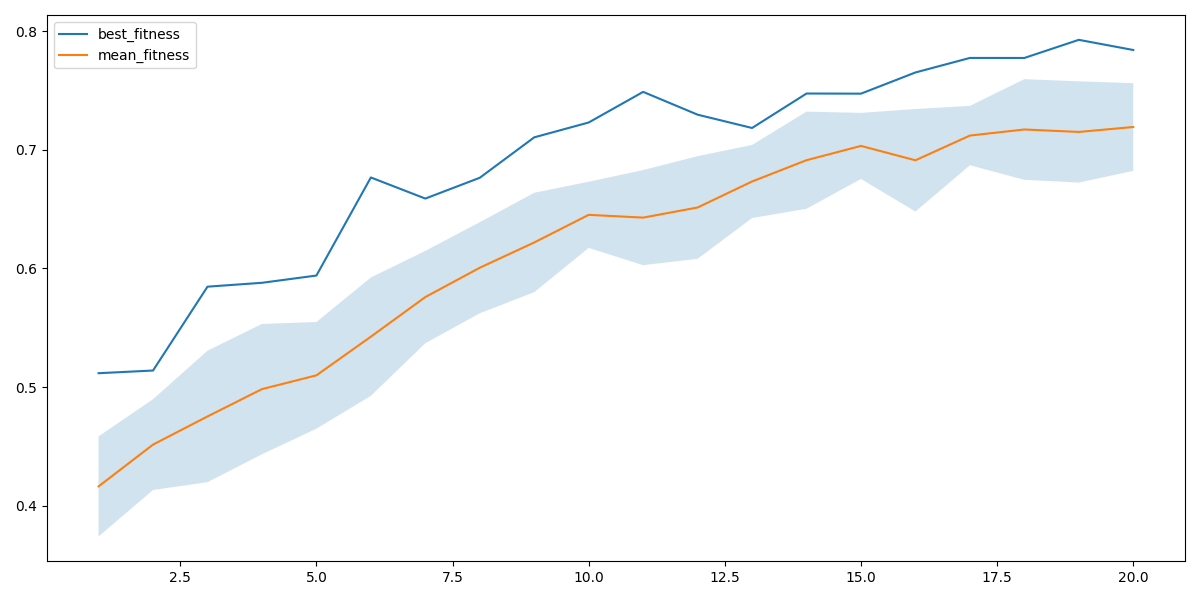
\includegraphics[width=\textwidth,height=0.62\textheight,keepaspectratio]{fitness_curves.png}
\end{columns}
\end{frame}

\begin{frame}{Official Melee Scoreboard}
\small
\begin{table}
\centering
\begin{tabular}{lrrrr}
\toprule
\textbf{Bot} & \textbf{Rank} & \textbf{Total Score} & \textbf{Firsts} & \textbf{Bullet Damage} \\
\midrule
\rowcolor{softgold} Jacob3\_0 & 1 & 81,613 & 113 & 38,858 \\
SarsaBot & 2 & 70,785 & 68 & 33,950 \\
PPOBot & 3 & 37,644 & 19 & 19,100 \\
MeleeDQN & 4 & 19,131 & 0 & 910 \\
NeuroEvoMelee & 5 & 6,700 & 0 & 0 \\
\bottomrule
\end{tabular}
\end{table}

\begin{block}{Result}
Across the longer logged melee scoring, Jacob3\_0 led total score, first-place rounds, and bullet damage.
\end{block}
\end{frame}

\begin{frame}{Win Rate Comparison}
\centering
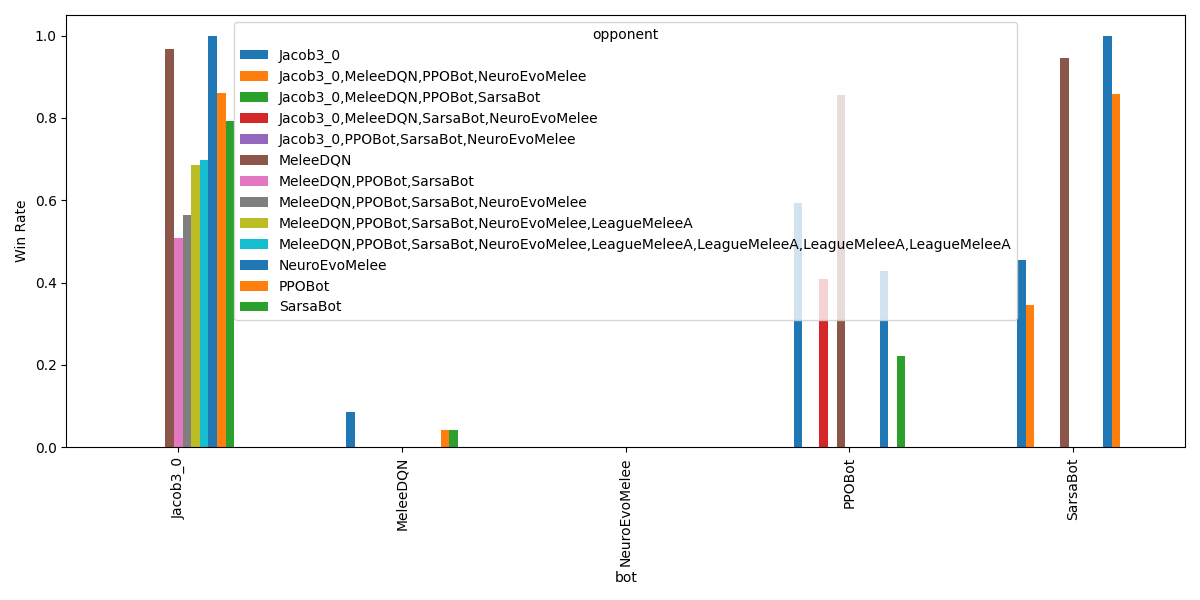
\includegraphics[width=0.94\textwidth,height=0.73\textheight,keepaspectratio]{win_rate_bar_chart.png}
\end{frame}

\begin{frame}{Reward Curves}
\centering
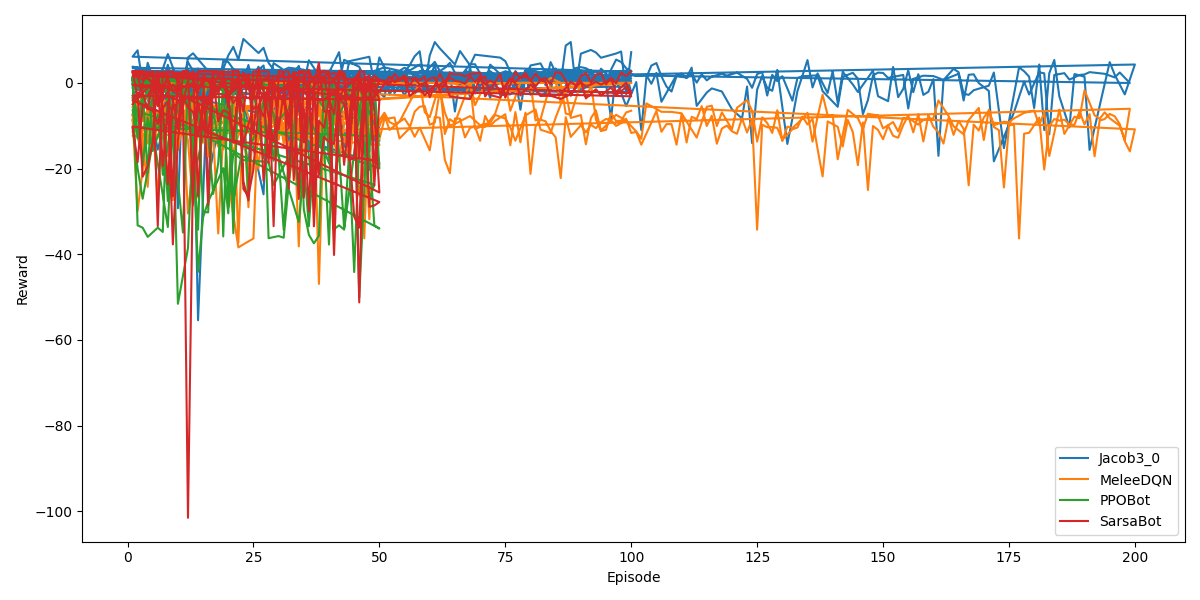
\includegraphics[width=0.94\textwidth,height=0.73\textheight,keepaspectratio]{reward_curves.png}
\end{frame}

\begin{frame}{Placement Heatmap}
\centering
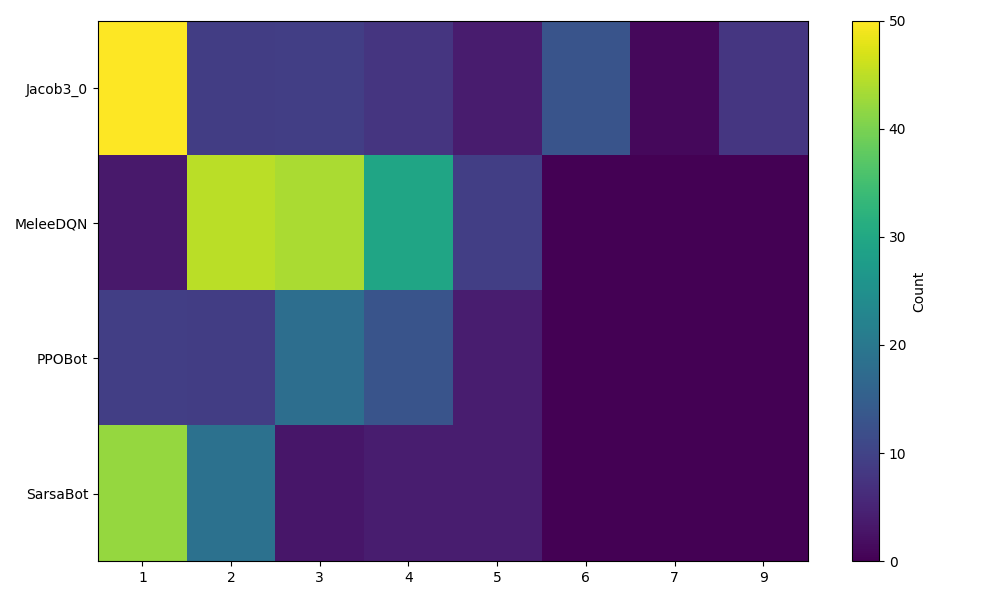
\includegraphics[width=0.88\textwidth,height=0.73\textheight,keepaspectratio]{placement_heatmap.png}
\end{frame}

\begin{frame}{What Worked}
\begin{itemize}
  \item Jacob3\_0's DQN setup gave the strongest final benchmark result.
  \item SARSA was a very useful baseline because it stayed competitive without neural-network complexity.
  \item PPO produced durable behavior, which is a good base for reward and action tuning.
  \item The log pipeline now captures episodes, summaries, state rows, reward curves, scoreboards, and failure notes.
\end{itemize}
\end{frame}

\begin{frame}{What Did Not Work Yet}
\begin{itemize}
  \item MeleeDQN learned little offense and collapsed in the final evaluation matrix.
  \item PPO survived but did not deal enough damage to win consistently.
  \item PPO++ does not yet have comparable logged benchmark summaries.
  \item NeuroEvoMelee fitness improved, but final battle behavior still had no reliable damage output.
  \item The April 28 stress test exposed a PyTorch in-place gradient issue during long training.
\end{itemize}
\end{frame}

\begin{frame}{Next Changes}
\begin{block}{Double DQN target}
\[
y_t=r_t+\gamma(1-d_t)Q_{\bar\theta}
\left(s_{t+1},\arg\max_{a'}Q_\theta(s_{t+1},a')\right)
\]
\end{block}

\begin{block}{Reward retuning}
\[
r_t = c_1D_{dealt} - c_2D_{taken} - c_3H_{wall}
+ c_4K + c_5W
\]
\end{block}

\small Tune the constants against a frozen validation suite instead of only judging from one run.
\end{frame}

\begin{frame}{Conclusion}
\begin{itemize}
  \item Ordered story: SARSA baseline, DQN attempt, Jacob3\_0 winner, PPO contender, PPO++ next.
  \item Jacob3\_0 finished first in the logged melee scoreboard and dominated most 1v1 evaluations.
  \item SARSA earned the clearest second-place story; PPO needs more reward/action work.
  \item The next fair test is to run PPO++ through the exact same benchmark matrix.
\end{itemize}
\end{frame}

\end{document}
